% !TEX root = ../../main.tex
\section{Data Gathering}\label{sec:data_gathering}
\TODO{Determine subjects:}
\begin{enumerate}
  \item Roemer?
  \item Jos?
  \item Marc
\end{enumerate}
For our data sets of real world activities we have sampled both in- and outdoor activities.
The subjects performing the activities are three males, of an age around 25.
We have used two series of recordings.
The first series consists of various outdoor recordings with segments of walking, running and standing.
Some activities are performed in a straight line, whilst others are performed around corners or in a wide circular direction.
The second series consists mainly of walking up and down the stairs, with small vertical parts between the segments.
The stairs are all in a circular shape.

\subsection{Outdoor straight lines}\label{subsec:outdoor_straight}
The first series of outdoor performed activities consist of walking and running segments in a straight line.
Halfway the recording is a $180^{\circ}$ turn.
The activities consist of standing still, walking and running (both jogging and sprinting).
The plots of \Cref{fig:plots_subject_2} shows the recordings of Subject $2$.
The recorded metrics originate from the accelerometer, rotational and magnetometer sensors.
The solid black lines indicate manually annoted change points, the dashes lines indicate the closest discovered change point.
A still from the video recording, showing Subject $2$ performing a (sprinting) run segment, is in \Cref{fig:stills_subject_2_sprinting}.


% \begin{center}\begin{table}
%   \begin{tabulary}{\textwidth}{|l|c|c|}
%     \hline
%     \multicolumn{3}{|c|}{Subj 1, run 1} \\
%     \hline \hline
%     Act. & Ann. & Disc. \\
%     \hline
%     Still & 0 & *0* \\
%     \hline
%     Shake & 3.5 & *3.5* \\
%     \hline
%     Still & 4.2 & *4.2* \\
%     \hline
%     In pocket & 5.5 & *5.5* \\
%     \hline
%     Walk & 7 & *7* \\
%     \hline
%     Run & 10 & *10* \\
%     \hline
%     Walk & 14 & *14* \\
%     \hline
%     Run & 17.2 & *17.2* \\
%     \hline
%     Walk & 22.1 & *22.1* \\
%     \hline
%     Turn CCW & 23.5 & *23.5* \\
%     \hline
%     Walk & 24.2 & *24.2* \\
%     \hline
%     Run (sprint) & 28 & *28* \\
%     \hline
%     Run & 31 & *31* \\
%     \hline
%     Walk & 33 & *33* \\
%     \hline
%     Run & 35.5 & *35.5* \\
%     \hline
%     Walk & 39 & *39* \\
%     \hline
%     Out pocket & 41 & *41* \\
%     \hline
%     Still & 43 & *43* \\
%     \hline
%     \hline
%     \multicolumn{2}{|l|}{Ratio Total CPs} & 3.2 \\
%     \hline
%     \multicolumn{2}{|l|}{Sum of differences} & 12.341 \\
%     \hline
%   \end{tabulary}
%   \caption[Performed activities subject 1 run 1]{The outdoor series performed activities by subject 1, run 1.}
%   \label{tab:outdoor_series}
% \end{table}\end{center}

% ===== OUTDOOR FREE ACTIVITIES ========
\subsection{Outdoor free}\label{subsec:outdoor_free}
The second series of outdoor recordings consist of more free-form activities.
The performed activities consist, as with the first set, of standing, walking, and running.
Furthermore, the segments are performed in a circular manner.
\eg the running activities are performed around a fountain with an estimated diameter of 10 meters.
The plots of the recordings of Subject, for the accelerometer, rotation, and magnetometer are shown in...
\TODO{Add plots}
For Subject~$1$ the still of the video recordings are in the upper row of \Cref{fig:stills_subject_1_and_2}, for Subject~$2$ in the lower row.

\begin{figure}
  \centering
  \begin{subfigure}[b]{1\textwidth}
    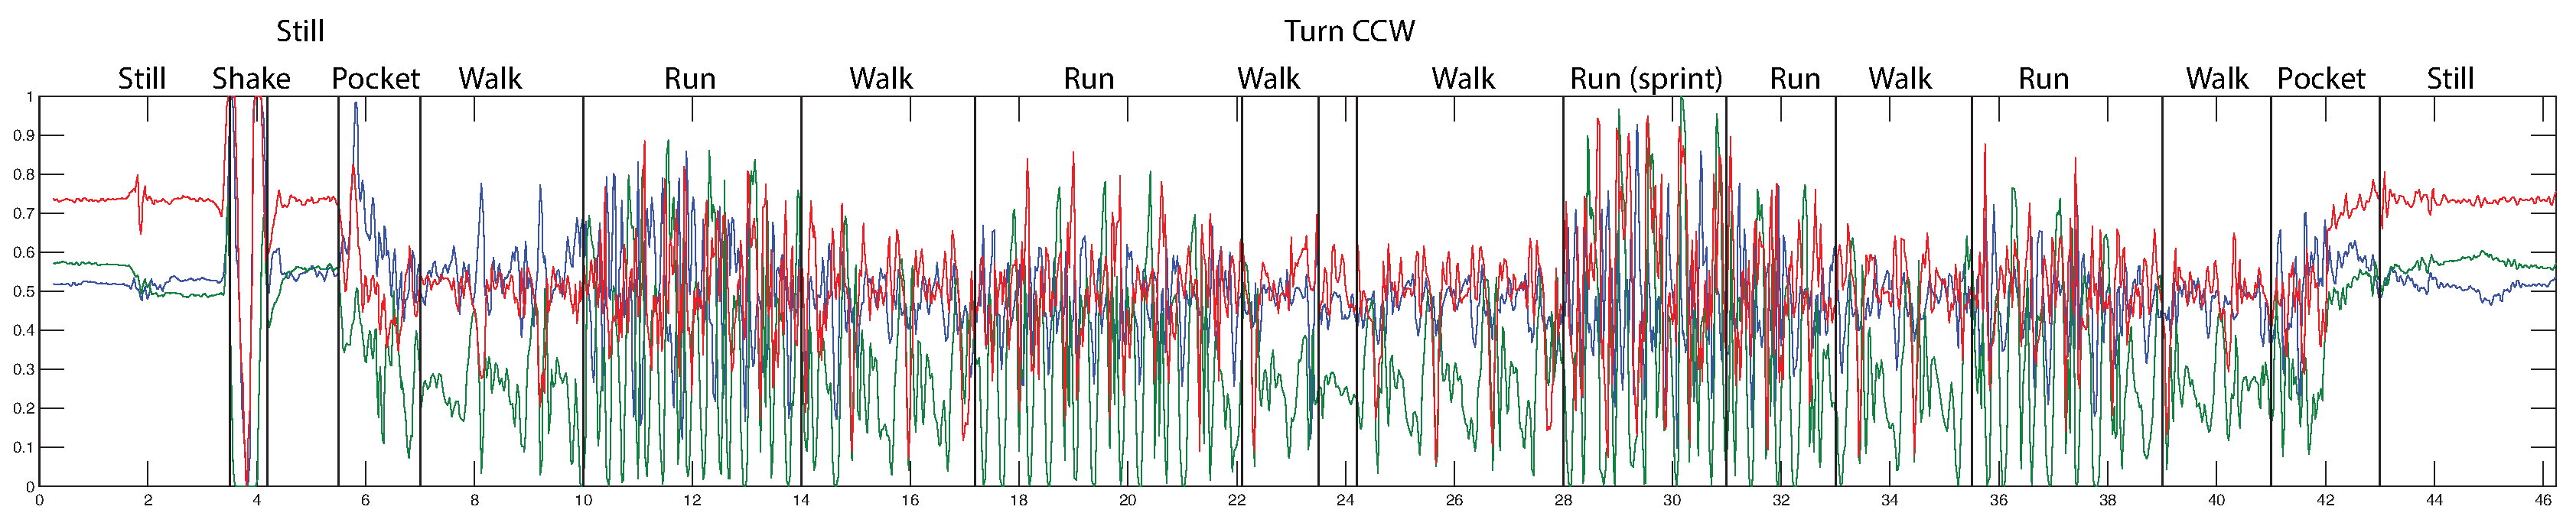
\includegraphics[width=\textwidth]{./Figures/chapter6/data_collection/run-1-walk-run-roemer/data_plot_acc_annotated.eps}
    \caption{Accelerometer}
    \label{fig:recording_subject_1_run_1_accelerometer}
  \end{subfigure}

  \begin{subfigure}[b]{1\textwidth}
    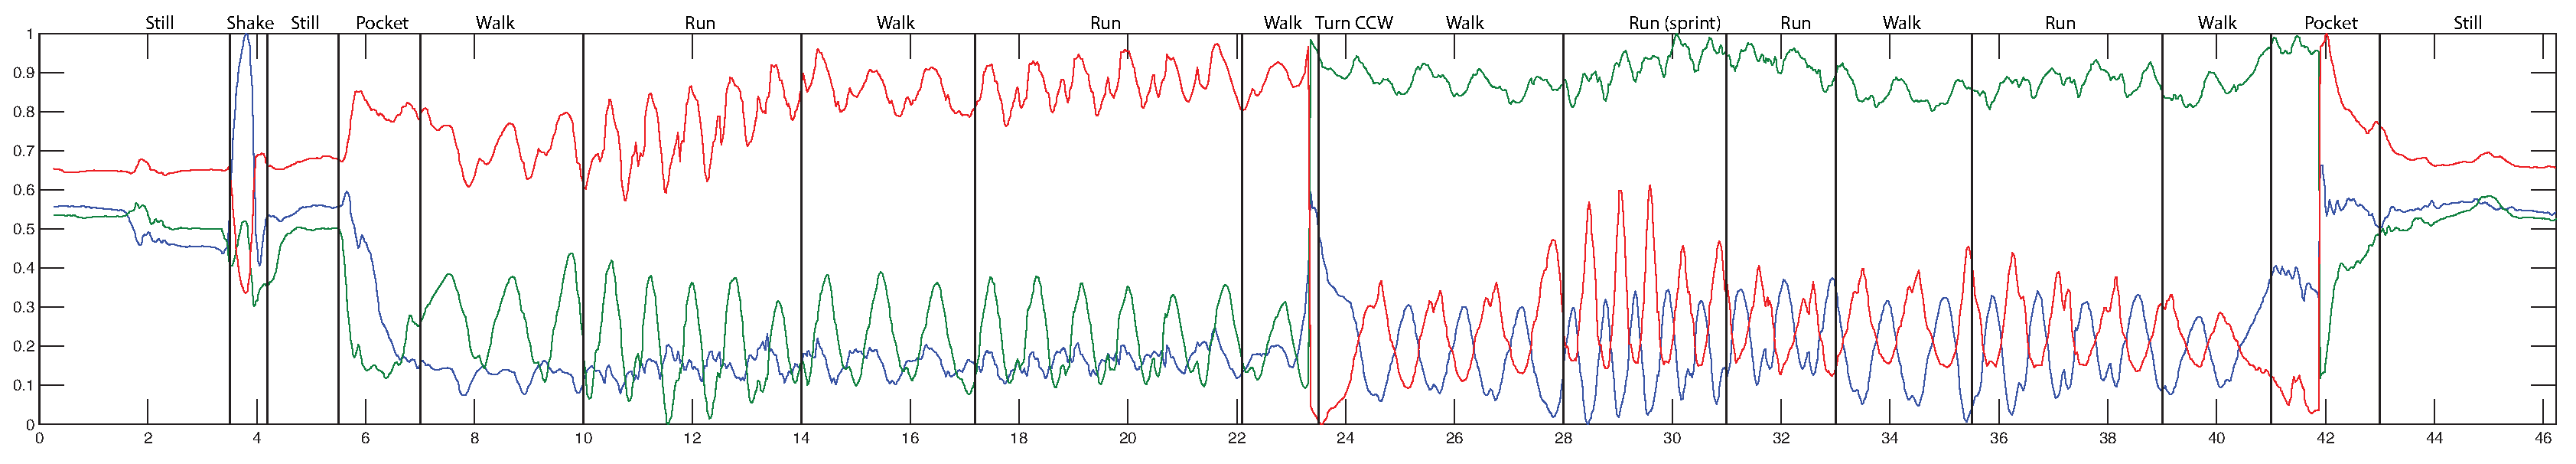
\includegraphics[width=\textwidth]{./Figures/chapter6/data_collection/run-1-walk-run-roemer/data_plot_rot_annotated.eps}
    \caption{Rotation}
    \label{fig:recording_subject_1_run_1_rotation}
  \end{subfigure} \\

  \begin{subfigure}[b]{1\textwidth}
    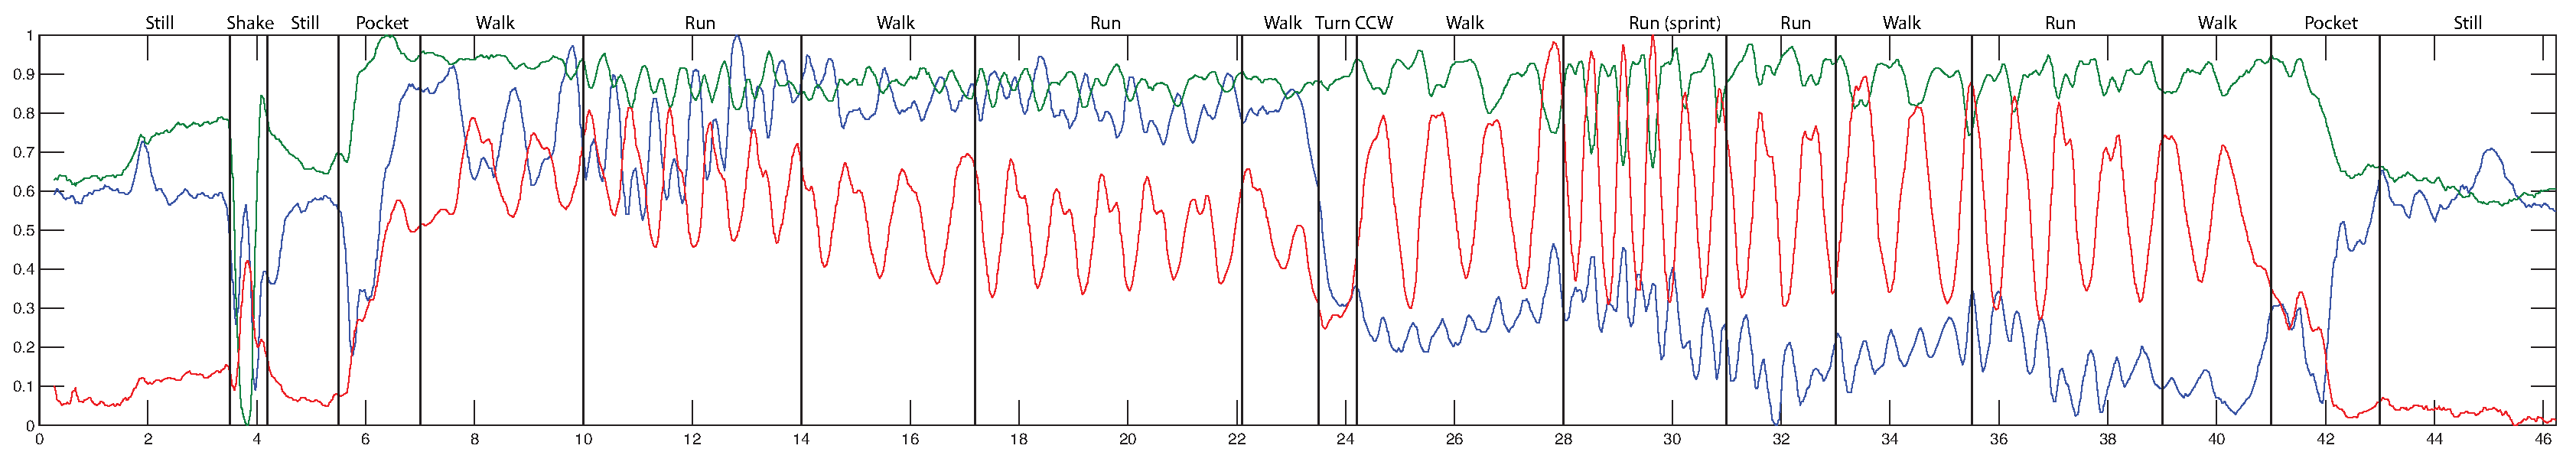
\includegraphics[width=\textwidth]{./Figures/chapter6/data_collection/run-1-walk-run-roemer/data_plot_mag_annotated.eps}
    \caption{Magnetic Field}
    \label{fig:recording_subject_1_run_1_magnetic}
  \end{subfigure} \\
  \caption[Plots]{Annotated plots of a full recording performed by Subject~$2$. The vertical lines are manually determined change points. The label above each segment indicates the current performed activity.}\label{fig:plots_subject_2}
\end{figure}


\begin{figure}
  \centering
  \begin{subfigure}[b]{0.2\textwidth}
    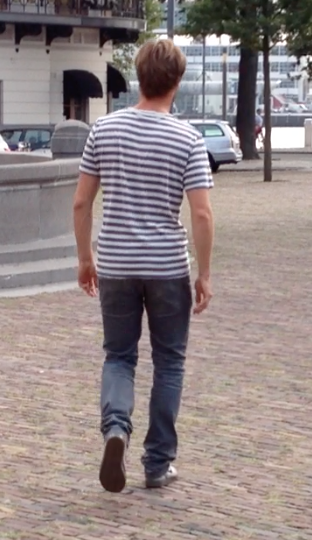
\includegraphics[width=\textwidth]{./Figures/chapter6/data_collection/stills/jos_walking.png}
    \caption{Walking}
    \label{fig:stills_subject_2_walking}
  \end{subfigure}%
  \qquad \qquad \qquad
  \begin{subfigure}[b]{0.2\textwidth}
    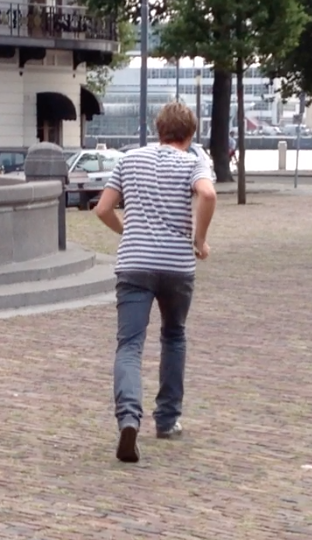
\includegraphics[width=\textwidth]{./Figures/chapter6/data_collection/stills/jos_cp_walk-run.png}
    \caption{Change point}
    \label{fig:stills_subject_2_change_point}
  \end{subfigure}
  \qquad \qquad \qquad
  \begin{subfigure}[b]{0.2\textwidth}
    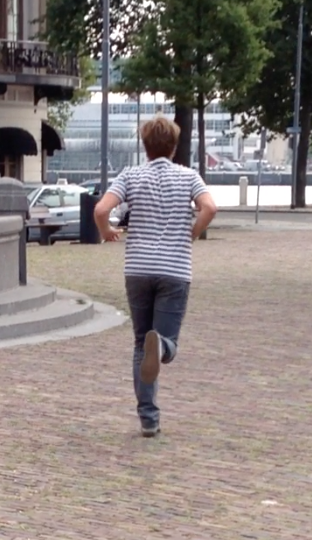
\includegraphics[width=\textwidth]{./Figures/chapter6/data_collection/stills/jos_run_2.png}
    \caption{Running}
    \label{fig:stills_subject_2_running}
  \end{subfigure}
  \par\bigskip
  \begin{subfigure}[b]{0.2\textwidth}
    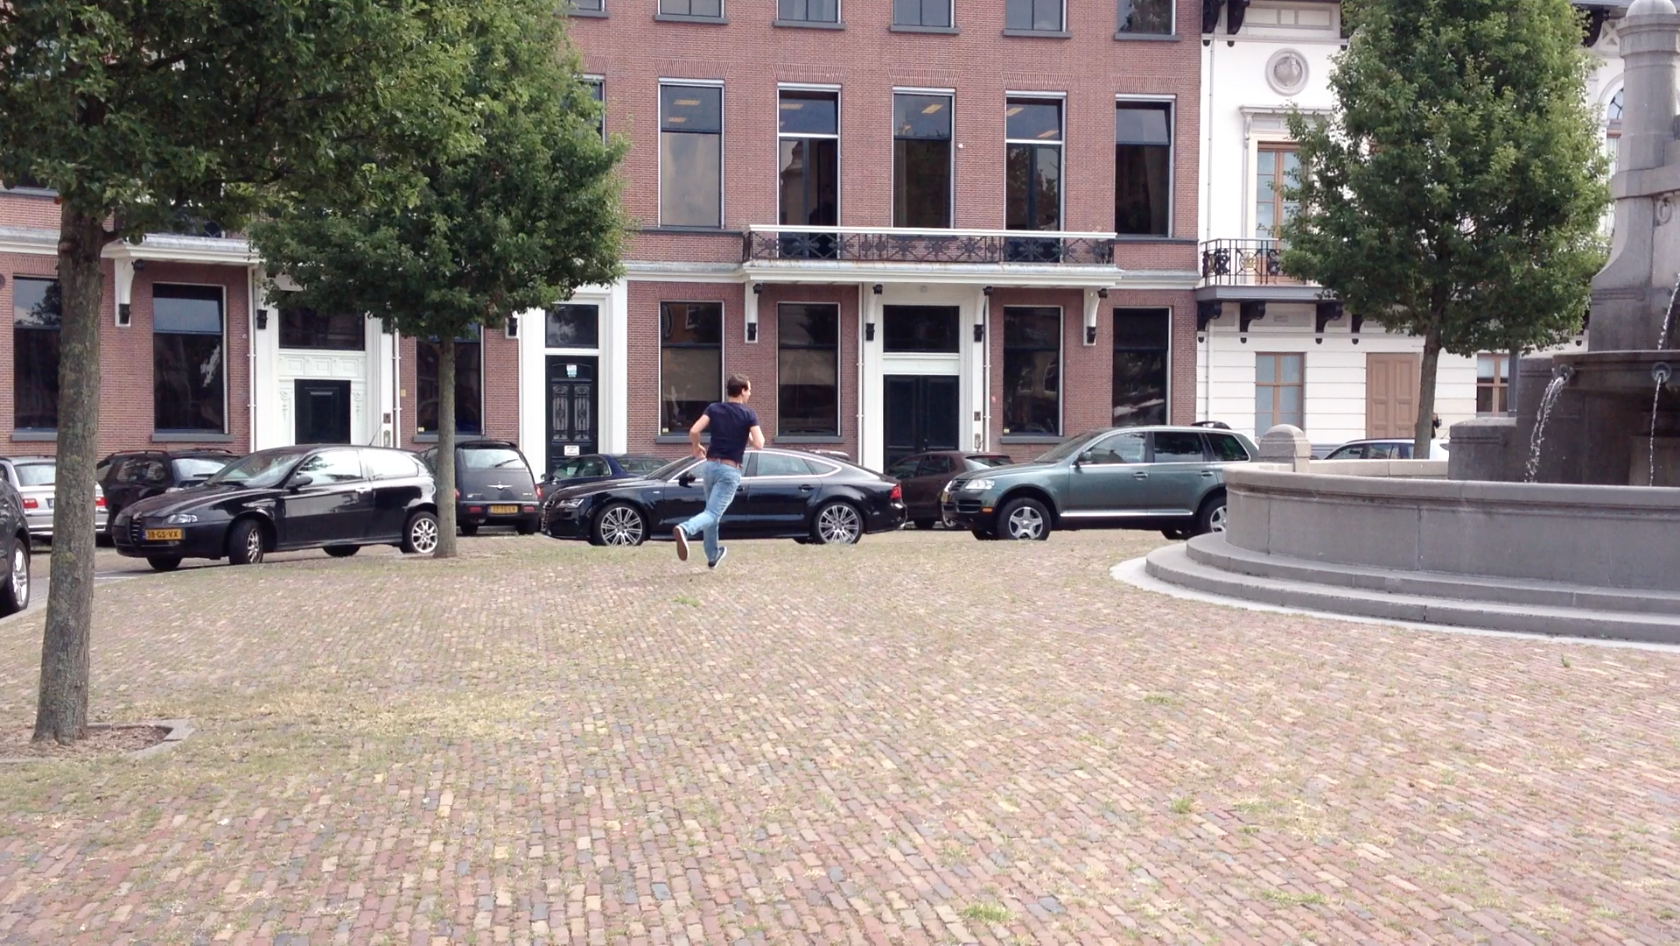
\includegraphics[width=\textwidth]{./Figures/chapter6/data_collection/stills/roemer_run_cw.png}
    \caption{Running CW}
    \label{fig:stills_subject_1_running_clockwise}
  \end{subfigure}
  \qquad \qquad \qquad
  \begin{subfigure}[b]{0.2\textwidth}
    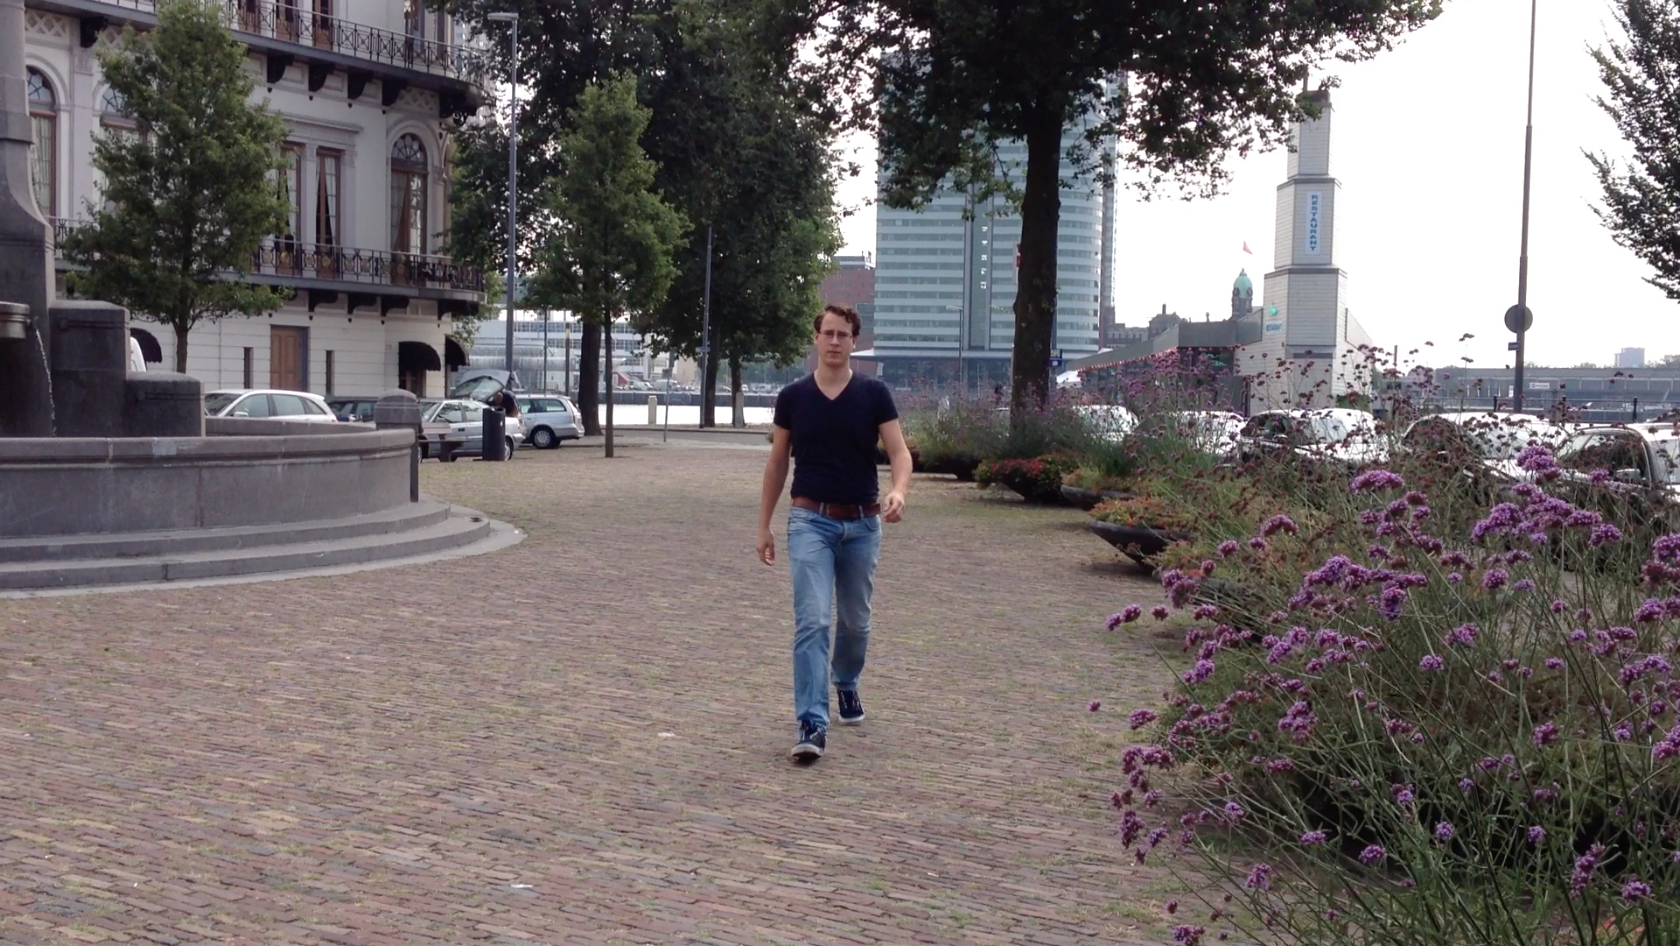
\includegraphics[width=\textwidth]{./Figures/chapter6/data_collection/stills/roemer_walk.png}
    \caption{Walking}
    \label{fig:stills_subject_1_walking}
  \end{subfigure}
  \qquad \qquad \qquad
  \begin{subfigure}[b]{0.2\textwidth}
    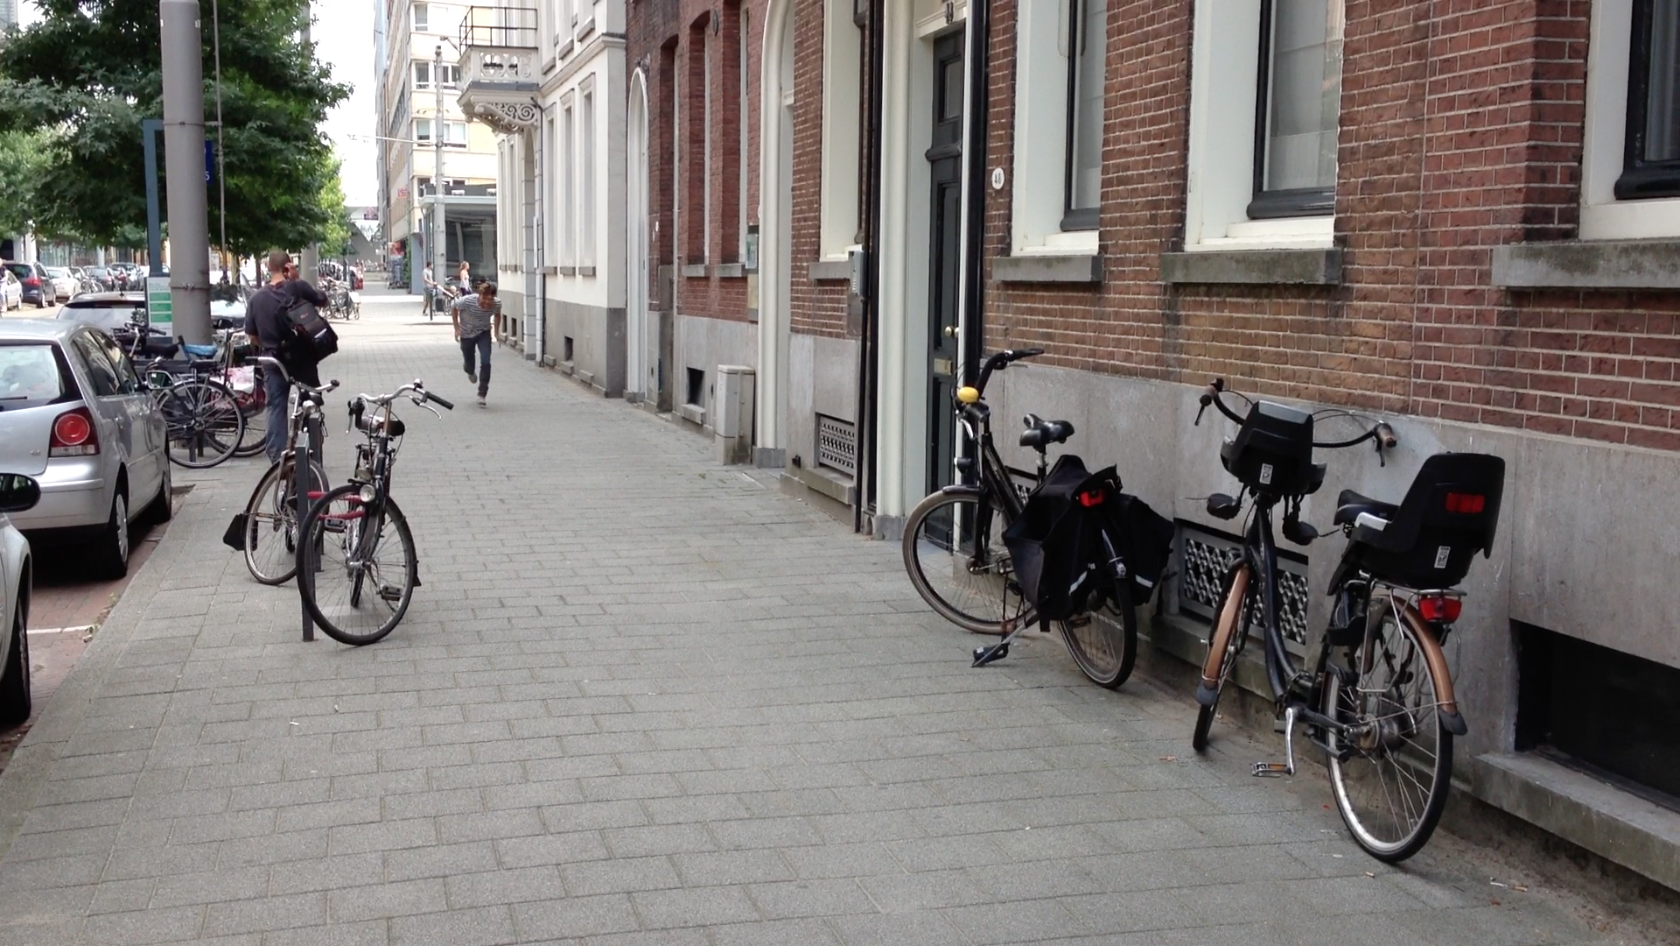
\includegraphics[width=\textwidth]{./Figures/chapter6/data_collection/stills/jos_sprint.png}
    \caption{Sprintng}
    \label{fig:stills_subject_2_sprinting}
  \end{subfigure}
  \caption[Stills subject 2]{Stills of video recordings during performing of the outdoor activities of walking and running. \Cref{fig:stills_subject_2_change_point} shows the change point between the two activities. \Cref{fig:stills_subject_1_running_clockwise} shows the running in clockwise motion.}\label{fig:stills_subject_1_and_2}
\end{figure}

\subsection{Indoor stairs}\label{subsec:indoor_stairs}
The final series of activities recorded consist of walking up and down the stairs, indoor.
The stairs are shaped in an semi-circular form, with a small vertical segment on each floor.
The still of \Cref{fig:stills_subject_3_downstairs} illustrates the circular shape of the stairs.
In \Cref{fig:stills_subject_3_upstairs} the small flat segment is visible.
Between the stairs the subject walked in a hallway with a $180^{\circ}$ counter-clockwise turn, as shown in \Cref{fig:stills_subject_3_walking}.
The recorded sensor data of the performed activities are visible in the plots of \Cref{fig:data_gathering_run_3_rot,fig:data_gathering_run_3_mag,fig:data_gathering_run_3_acc}.

\begin{figure}
  \centering
  \begin{subfigure}[b]{0.3\textwidth}
    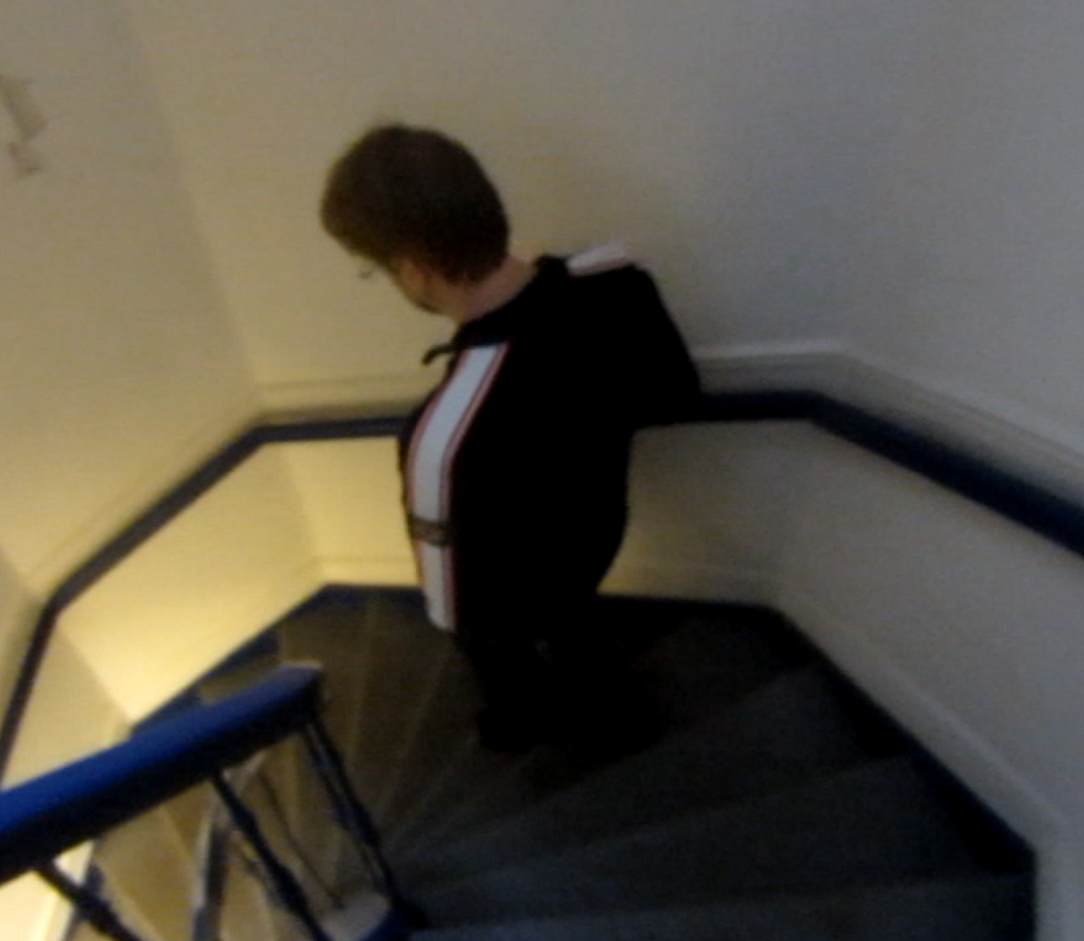
\includegraphics[width=\textwidth]{./Figures/chapter6/data_collection/stills/marc_downstairs.png}
    \caption{Downstairs}
    \label{fig:stills_subject_3_downstairs}
  \end{subfigure}%
  ~
  \begin{subfigure}[b]{0.3\textwidth}
    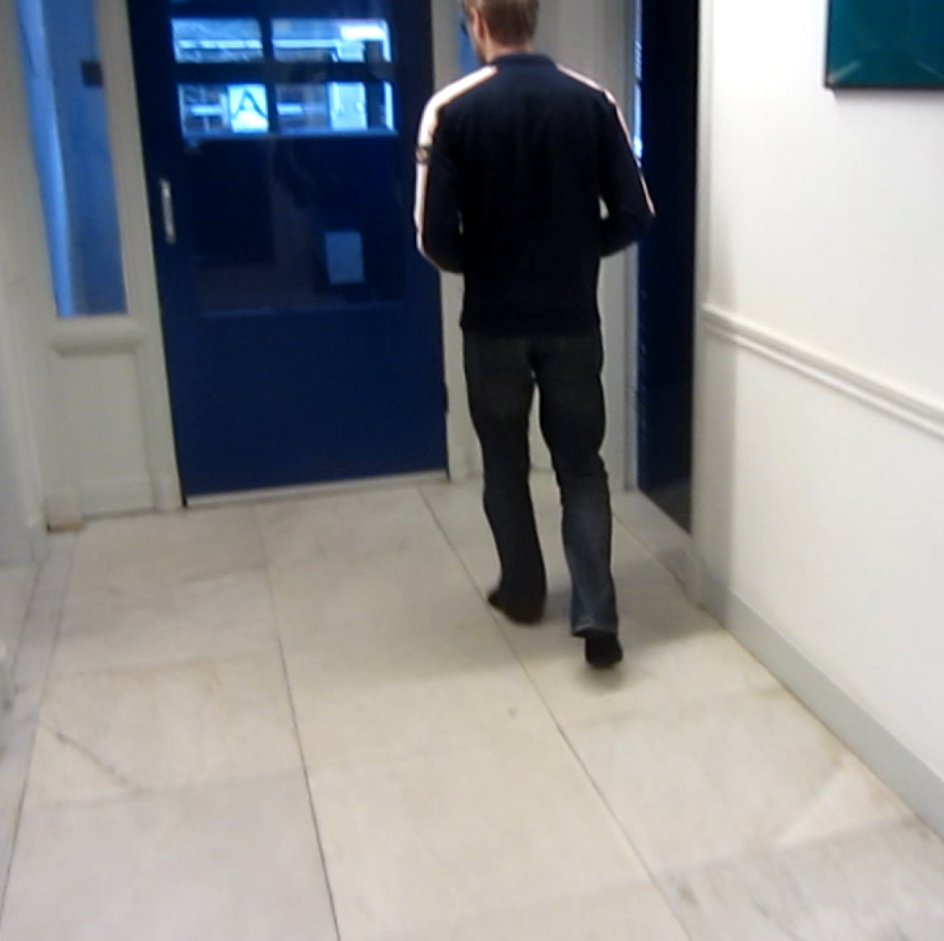
\includegraphics[width=\textwidth]{./Figures/chapter6/data_collection/stills/marc_walk.png}
    \caption{Walking}
    \label{fig:stills_subject_3_walking}
  \end{subfigure}
  ~
  \begin{subfigure}[b]{0.3\textwidth}
    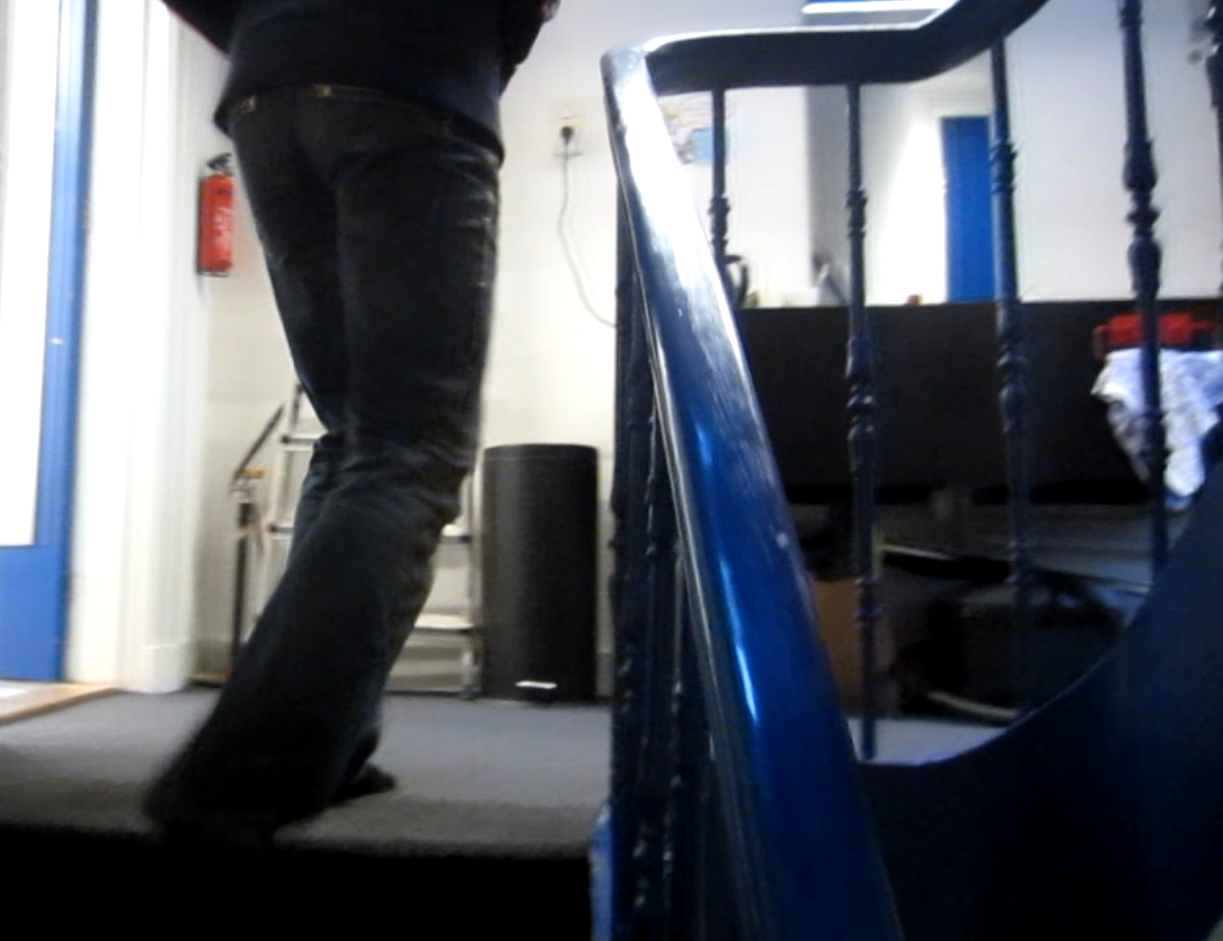
\includegraphics[width=\textwidth]{./Figures/chapter6/data_collection/stills/marc_stairs_up_walk.png}
    \caption{Upstairs}
    \label{fig:stills_subject_3_upstairs}
  \end{subfigure}
  \caption[Stills subject 3]{Stills of video recordings during performing of the indoor activities of walking, ascending and descending the stairs.}\label{fig:stills_subject_3}
\end{figure}

%---- Run 3: Stairs remco
\begin{figure}
  \centering
  \begin{subfigure}[b]{1\textwidth}
    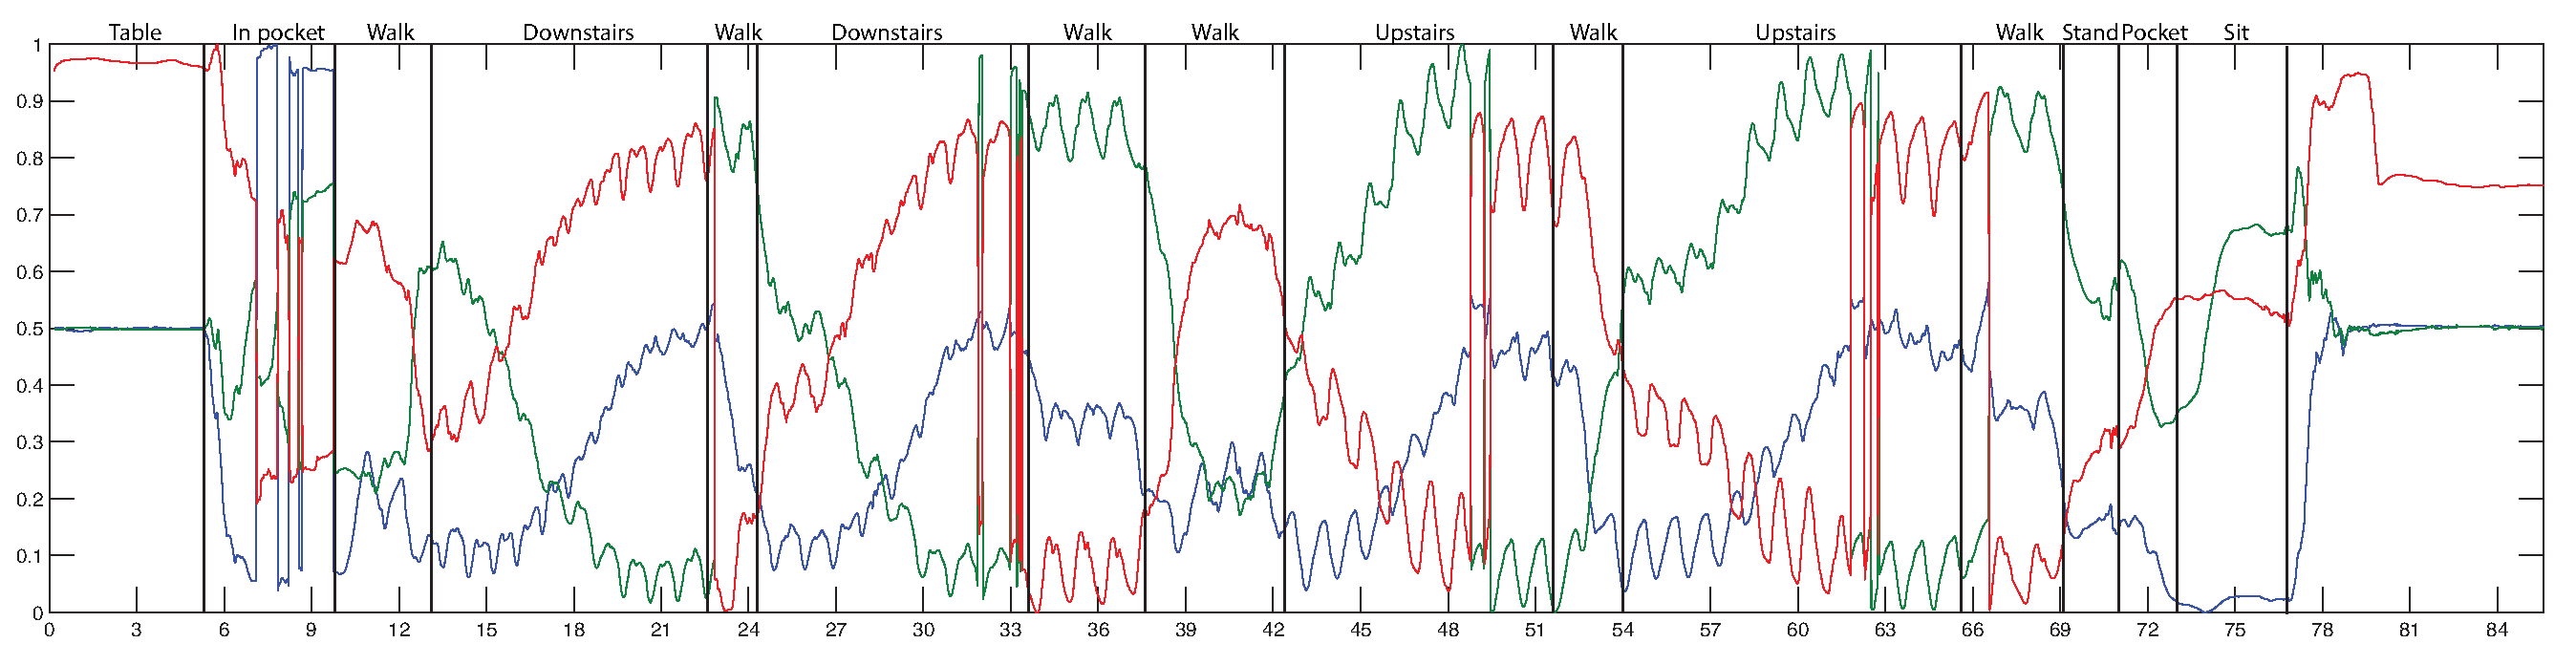
\includegraphics[width=\textwidth]{./Figures/chapter6/data_collection/stairs-1-marc/data_plot_rot_annotated.eps}
    \caption{Run 3: Indoor stairs Marc, rotation}
    \label{fig:data_gathering_run_3_rot}
  \end{subfigure} \\

  \begin{subfigure}[b]{1\textwidth}
    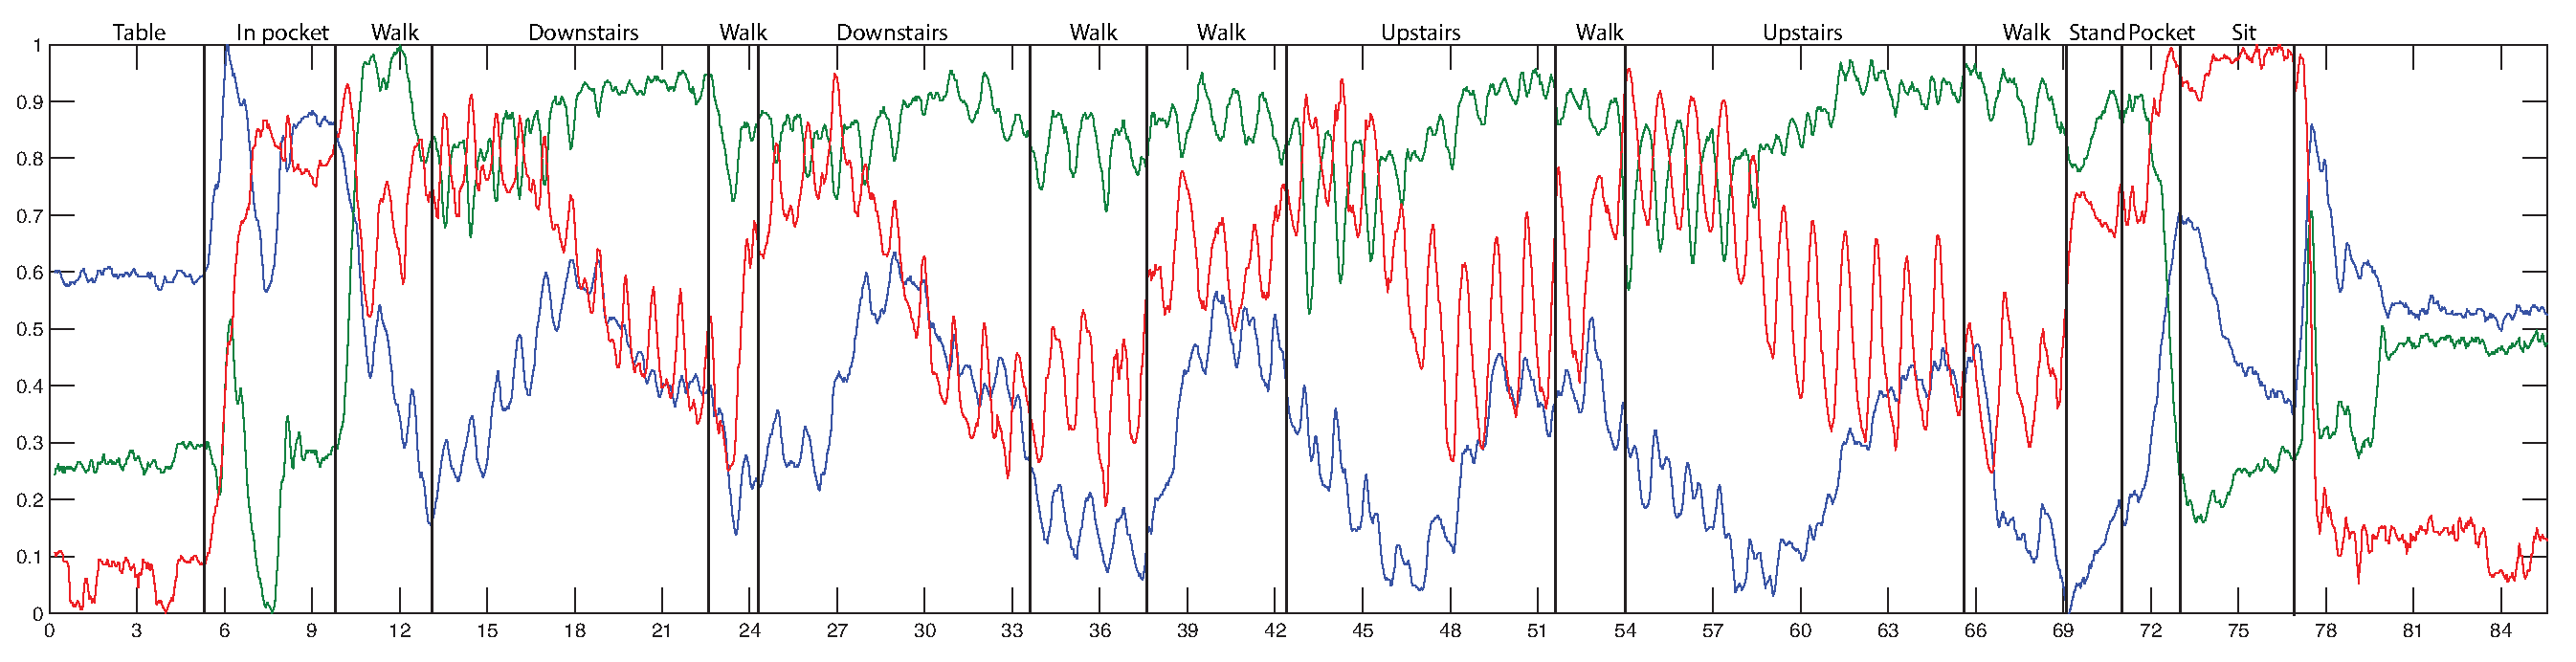
\includegraphics[width=\textwidth]{./Figures/chapter6/data_collection/stairs-1-marc/data_plot_mag_annotated.eps}
    \caption{Run 3: Indoor stairs Marc, Mag}
    \label{fig:data_gathering_run_3_mag}
  \end{subfigure} \\

  \begin{subfigure}[b]{1\textwidth}
    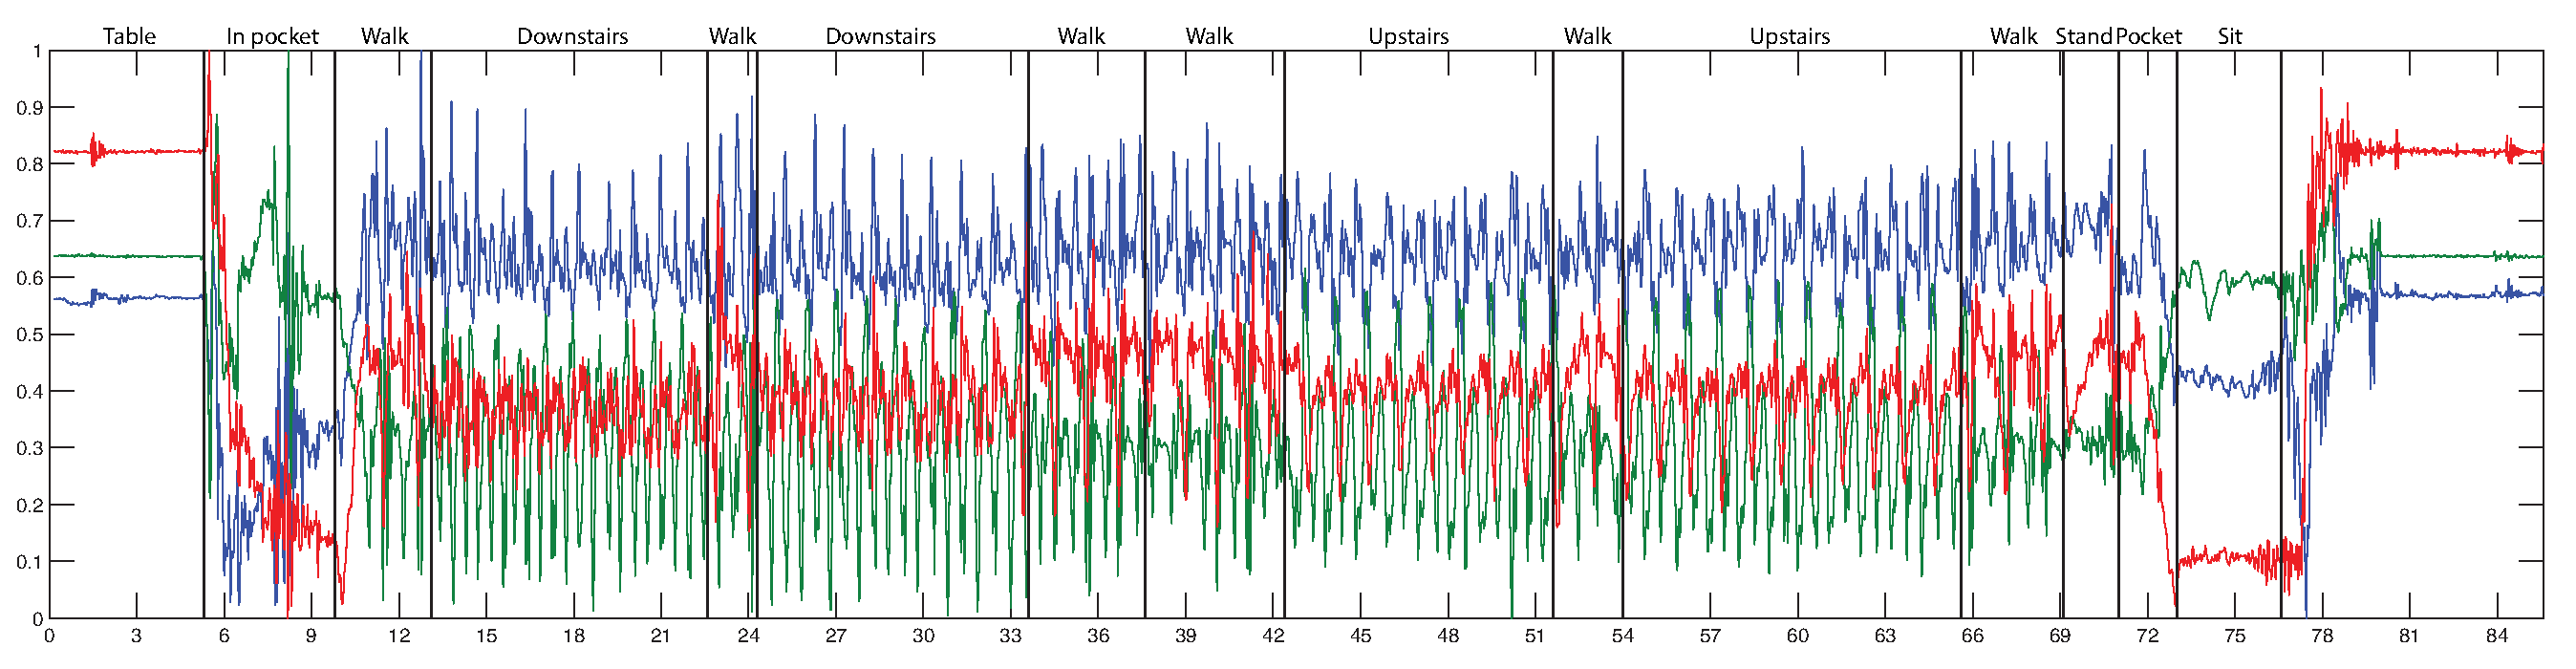
\includegraphics[width=\textwidth]{./Figures/chapter6/data_collection/stairs-1-marc/data_plot_acc_annotated.eps}
    \caption{Run 3: Indoor stairs Marc, accelerometer}
    \label{fig:data_gathering_run_3_acc}
  \end{subfigure}
  \caption[Plots subject 3]{Annotated plots of a full recording performed by Subject~$3$ while walking the stairs. The vertical lines are manually determined change points. The label above each segment indicates the current performed activity.}\label{fig:plots_subject_3}
\end{figure}